\documentclass[12pt,a4paper,leqno]{report}

\usepackage[T1]{fontenc}
\usepackage[english]{babel}
\usepackage{amsthm}
\usepackage{amsfonts}
\usepackage{amsmath}
\usepackage{amssymb}
\usepackage{tikz}
\usepackage{listings}

\newcommand{\R}{\mathbb{R}}
\newcommand{\C}{\mathbb{C}}
\newcommand{\Q}{\mathbb{Q}}
\newcommand{\N}{\mathbb{N}}
\newcommand{\No}{\mathbb{N}_0}
\newcommand{\Z}{\mathbb{Z}}
\newcommand{\diam}{\operatorname{diam}}

\theoremstyle{plain}
\newtheorem{equa}[equation]{Equation}
\newtheorem{lem}[equation]{Lemma}
\newtheorem{prop}[equation]{Proposition}
\newtheorem{cor}[equation]{Corollary}

\theoremstyle{definition}
\newtheorem{defi}[equation]{definition}
\newtheorem{conj}[equation]{Conjecture}
\newtheorem{example}[equation]{Example}

\theoremstyle{remark}
\newtheorem{note}[equation]{Note}

\pagestyle{plain}
\makeatletter
\renewcommand{\@seccntformat}[1]{}
\makeatother
\setcounter{page}{1}
\addtolength{\hoffset}{-1.15cm}
\addtolength{\textwidth}{2.3cm}
\addtolength{\voffset}{0.45cm}
\addtolength{\textheight}{-0.9cm}

\graphicspath{ {./figures/} }

\title{Data Analytics 2 - Predicting Brand Preference}
\author{Tuomo Kareoja}
\date{}

\begin{document}

\maketitle

\begin{table}[h!]
  \begin{center}
    \begin{tabular}{l|c|r}
      \textbf{Version Number} & \textbf{Changes} & \textbf{Date} \\
      \hline
      0.1 & Created basic outline without content & 01.08.2019\\
      0.2 & Added visualizations, printouts and text outlines & 02.08.2019\\
      0.9 & Better visualizations and more explanations. Abandoned ensemble models & 05.08.2019\\
    \end{tabular}
  \end{center}
\end{table}

\newpage

\section{Brand Preference with Predicted Missing Values}

\bigskip
{
    \centering
    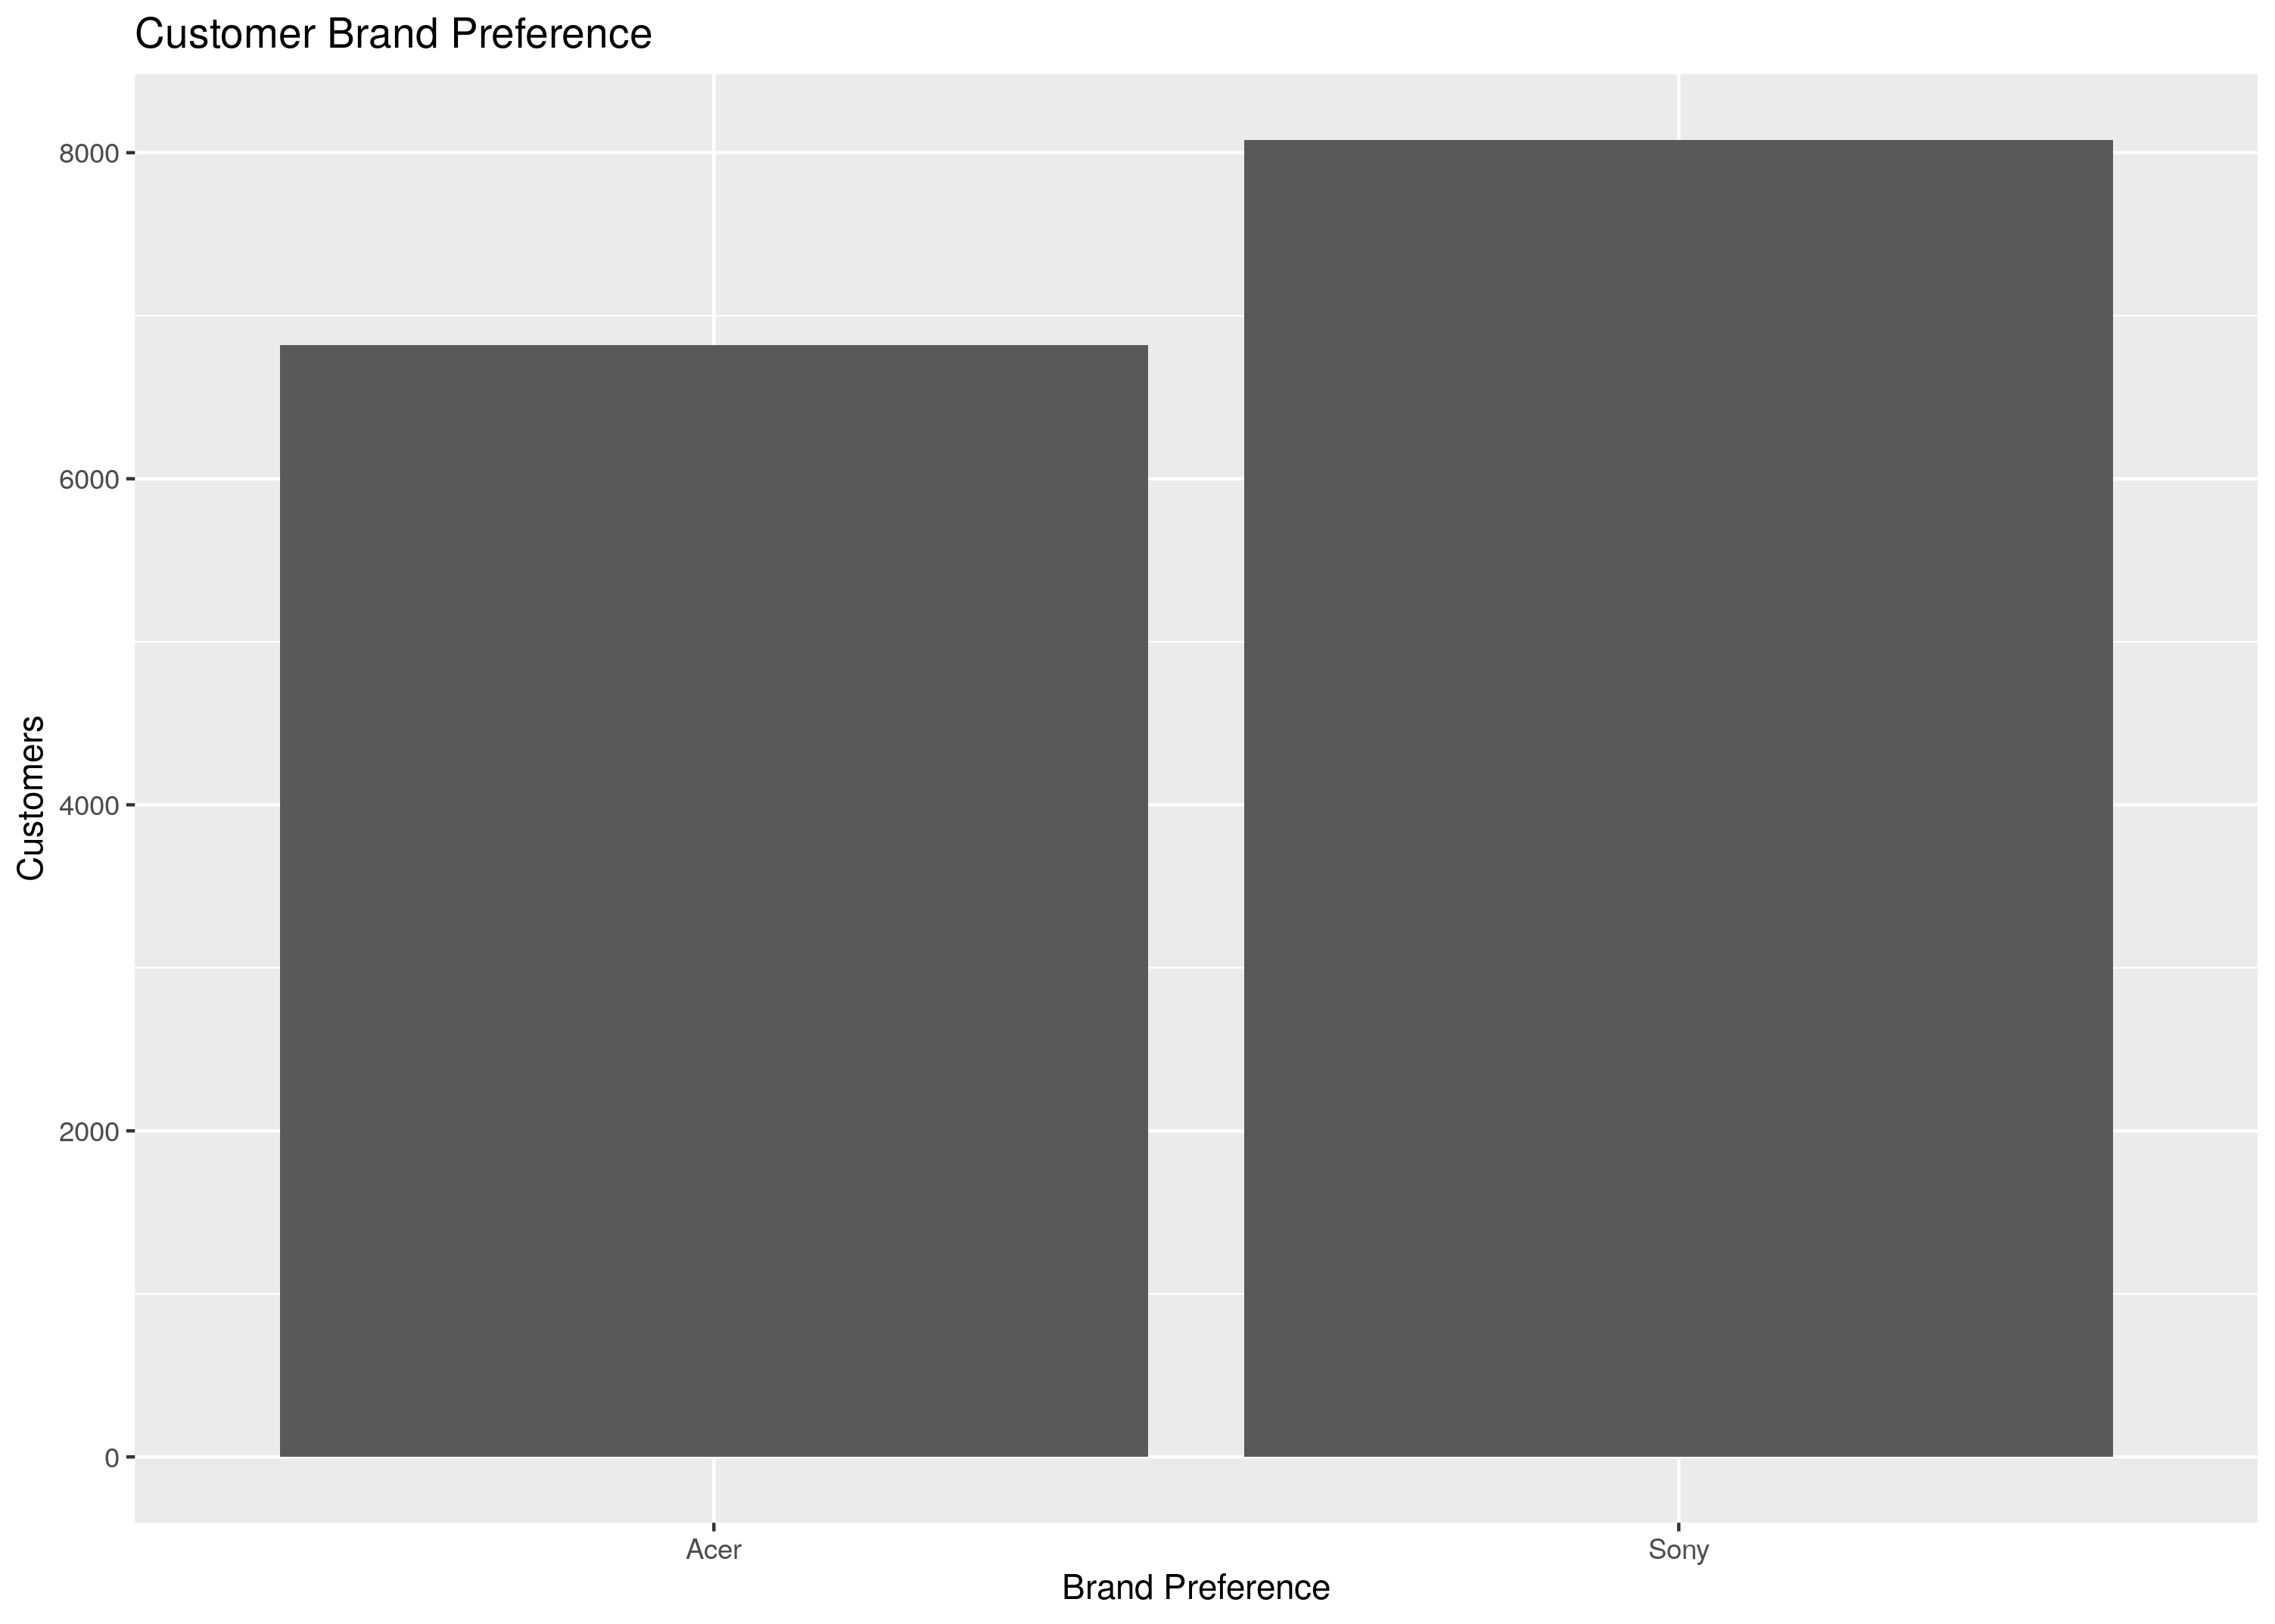
\includegraphics[width=\textwidth,height=\textheight,keepaspectratio]{brand_preference_plain.png}
    \par
}
\bigskip

These are results of the brand preference question after we added in our predictions. We can wee that Sony
is clearly the more preferred brand, but that the difference is not huge.

\bigskip
{
    \centering
    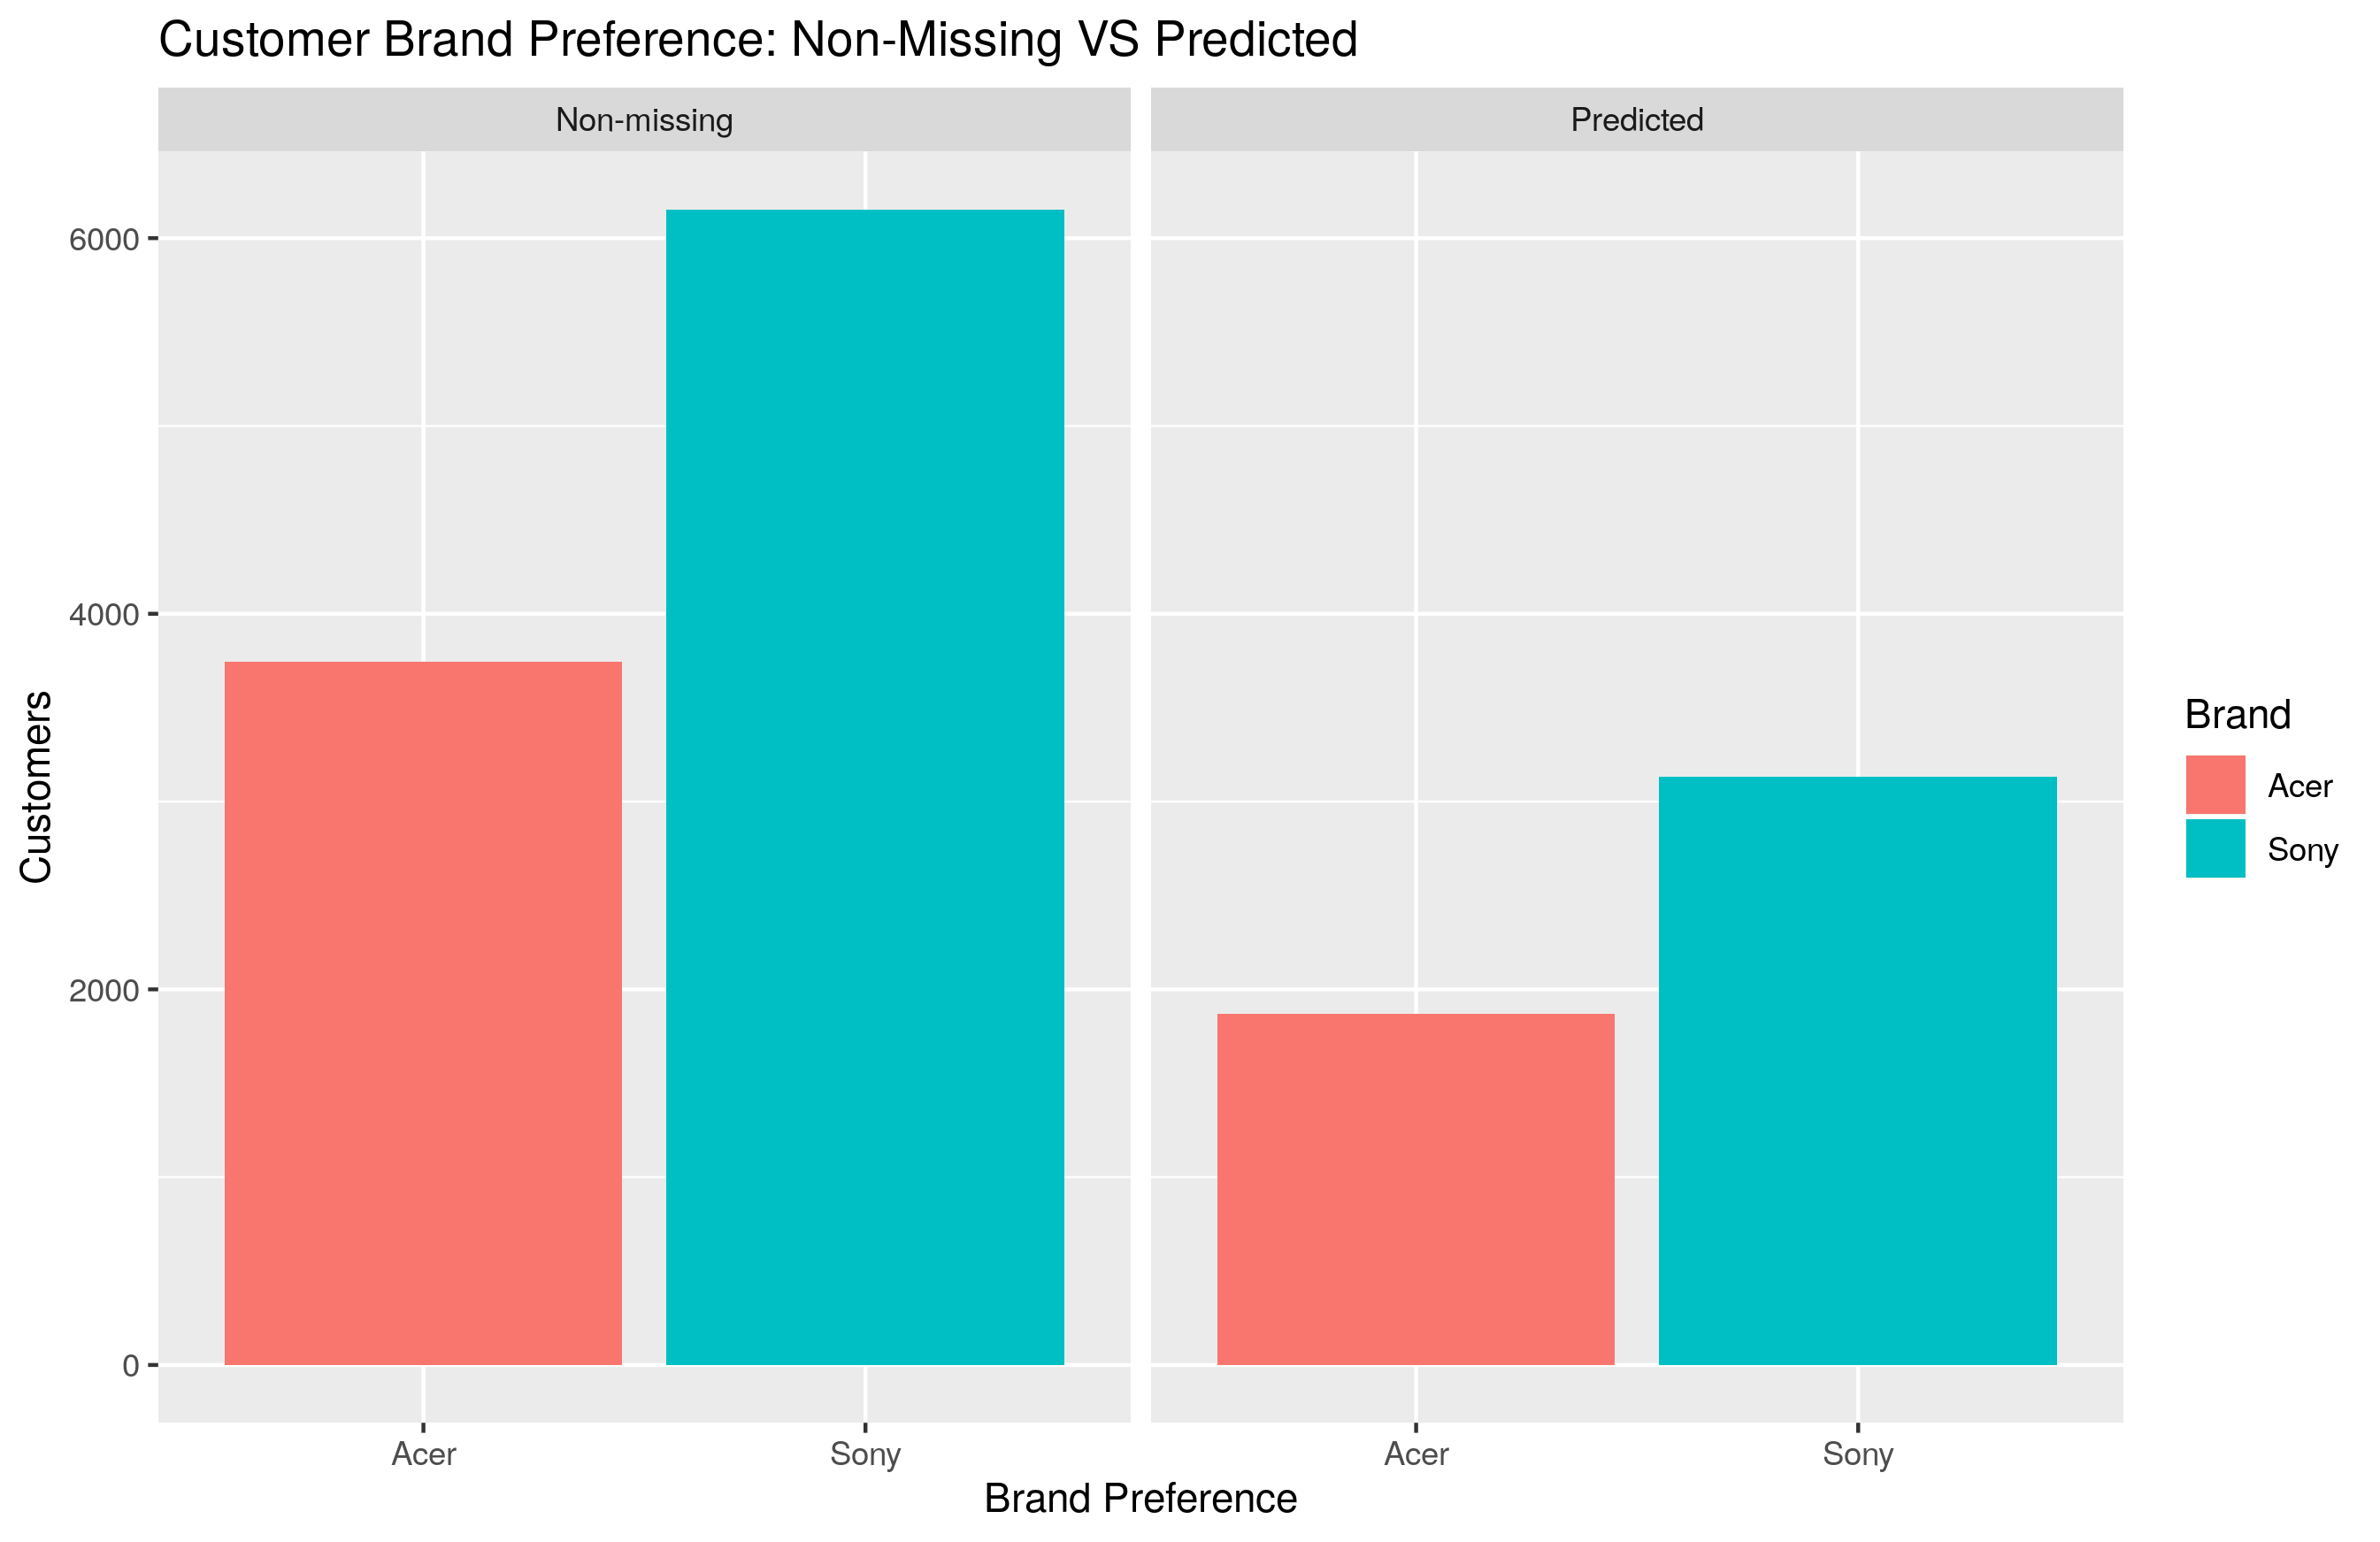
\includegraphics[width=\textwidth,height=\textheight,keepaspectratio]{brand_preference_marked.png}
    \par
}
\bigskip


Does look this is actually missing at random in relation to the brand preference.

TODO check percentages

Here we can see that if we would have just used the data without missing values our estimate of the difference
between the two brand would have been much bigger. In the predicted values there much more customers who are predicted
to prefer Acer more than Sony. Assuming that our model is correct, this means that the data about brand
preference is not missing at random and that using just the non-missing values would lead to quite biased
conclusions.


\section{Chosen Model and Its' Performance}

The model used for the predictions is a C5.0 classification tree. From the the graphs below we can see that
on all the important metrics this model performs really well with the Test set accuracy score being.
If we compare the test set and train set accuracy metric we can see that the model also seems to have almost no overfit.

\bigskip
{
    \centering
    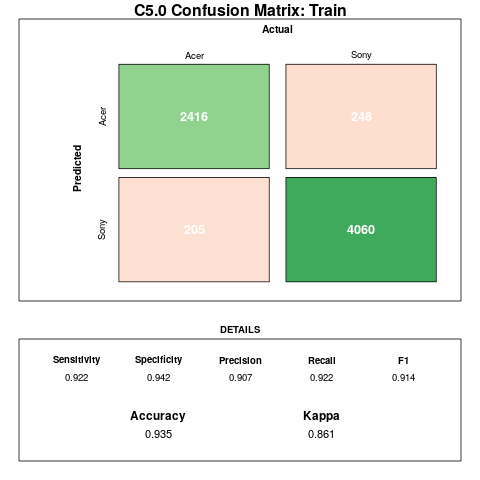
\includegraphics[width=\textwidth,height=\textheight,keepaspectratio]{cm_c5_train.png}
    \par
}
\bigskip

\bigskip
{
    \centering
    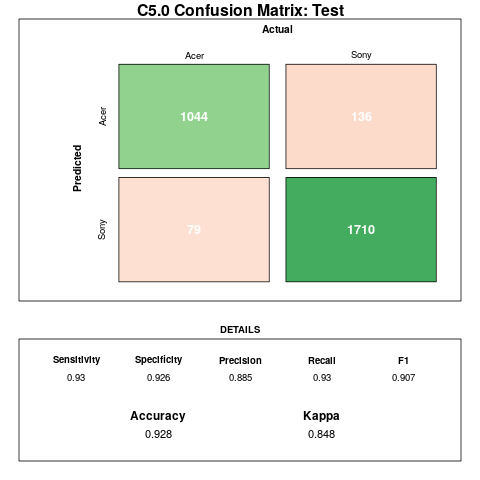
\includegraphics[width=\textwidth,height=\textheight,keepaspectratio]{cm_c5.png}
    \par
}
\bigskip

As the C5.0 decision tree is too complex to understandably visualize. We can instead look at the
relative model feature importances:

% \bigskip
% {
%     \centering
%     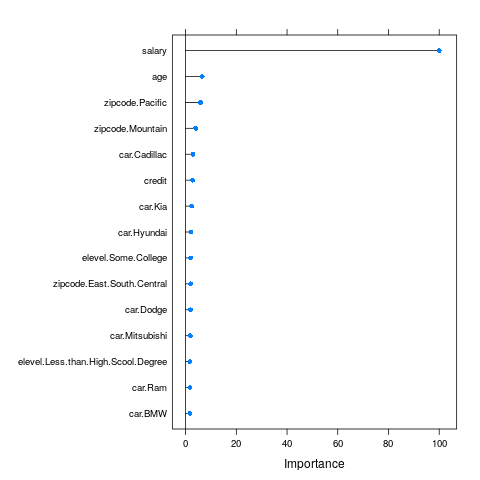
\includegraphics[width=\textwidth,height=\textheight,keepaspectratio]{c5_full_feature_importance.png}
%     \par
% }
% \bigskip

We can see that by far the most import variable is the salary of the customer. If we plot the distribution
of salary with the brand preference, we can see that there is clearly differences but that these
are quite complex and nonlinear and would have not been easily captured with a linear model.

\section{Model Comparison and Performance}

In total three different model types were tried: C5.0, Random Forest (RF) and Extreme Gradient Boosting (EGB).
All of these model are tree based models and all performed excellently. This made is quite problematic
to choose the best model.

From the cross validation boxplots we can see that all models perform very well in all metrics and it is hard to
decide which is the best:

\bigskip
{
    \centering
    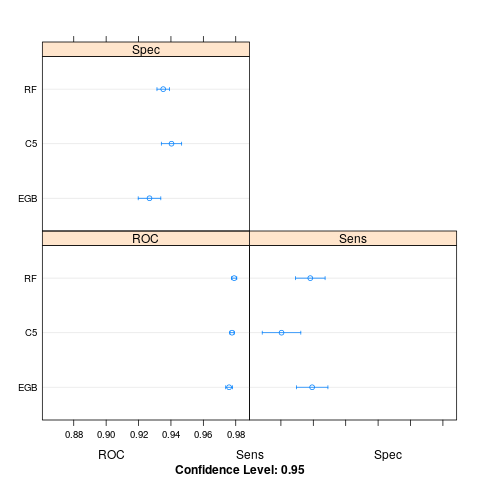
\includegraphics[width=\textwidth,height=\textheight,keepaspectratio]{dotplot_comparison.png}
    \par
}
\bigskip

The small differences between the models can best be seen in the ROC-curve:

\bigskip
{
    \centering
    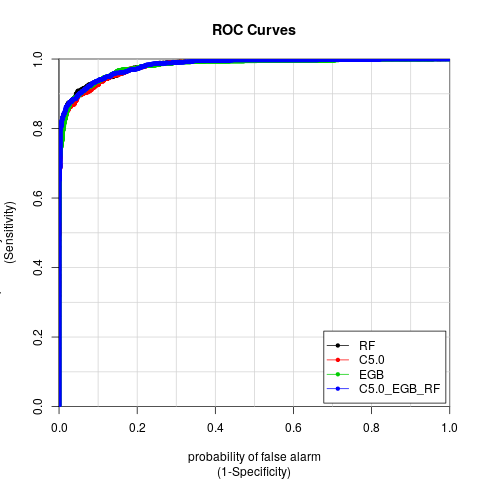
\includegraphics[width=\textwidth,height=\textheight,keepaspectratio]{AUC_comparison.png}
    \par
}
\bigskip

The models are almost indistinguishable, with our chosen C5.0 model maybe somewhat getting a head around
the optimal (Youden Index) point.

Random Forests confusion matrix test and train

\bigskip
{
    \centering
    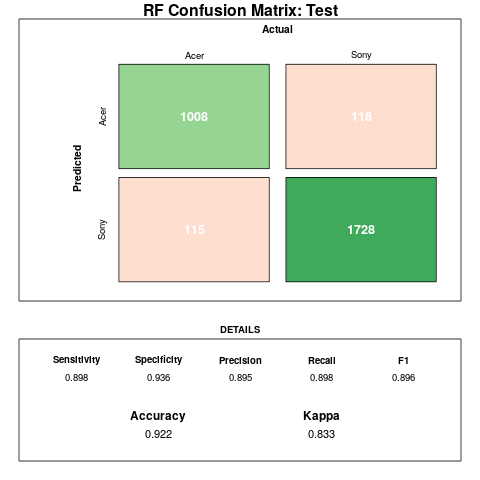
\includegraphics[width=\textwidth,height=\textheight,keepaspectratio]{cm_rf.png}
    \par
}
\bigskip

\bigskip
{
    \centering
    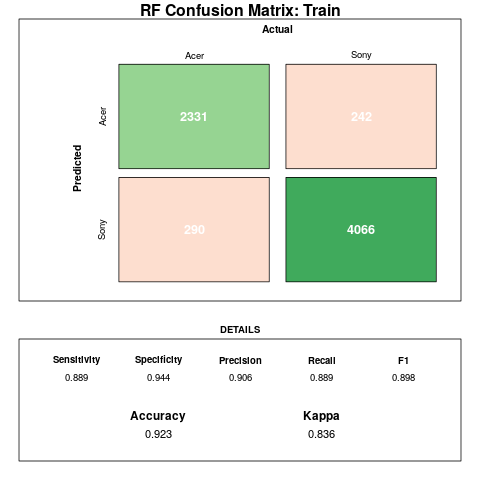
\includegraphics[width=\textwidth,height=\textheight,keepaspectratio]{cm_rf_train.png}
    \par
}
\bigskip

Extreme Gradient Boosting confusion matrix test and train

\bigskip
{
    \centering
    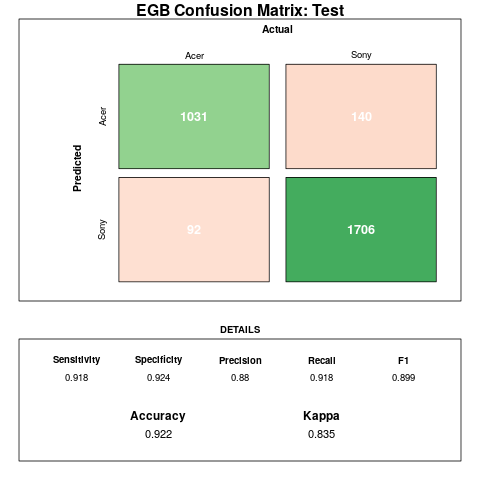
\includegraphics[width=\textwidth,height=\textheight,keepaspectratio]{cm_egb.png}
    \par
}
\bigskip

\bigskip
{
    \centering
    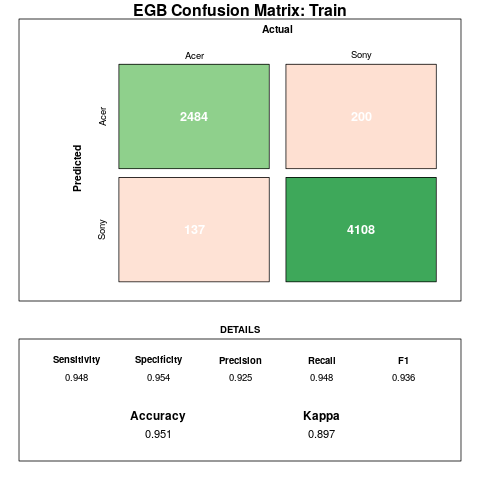
\includegraphics[width=\textwidth,height=\textheight,keepaspectratio]{cm_egb_train.png}
    \par
}
\bigskip

Model prediction correlation is quite low (cross validated scores don't line up neatly on the diagonal).

% \bigskip
% {
%     \centering
%     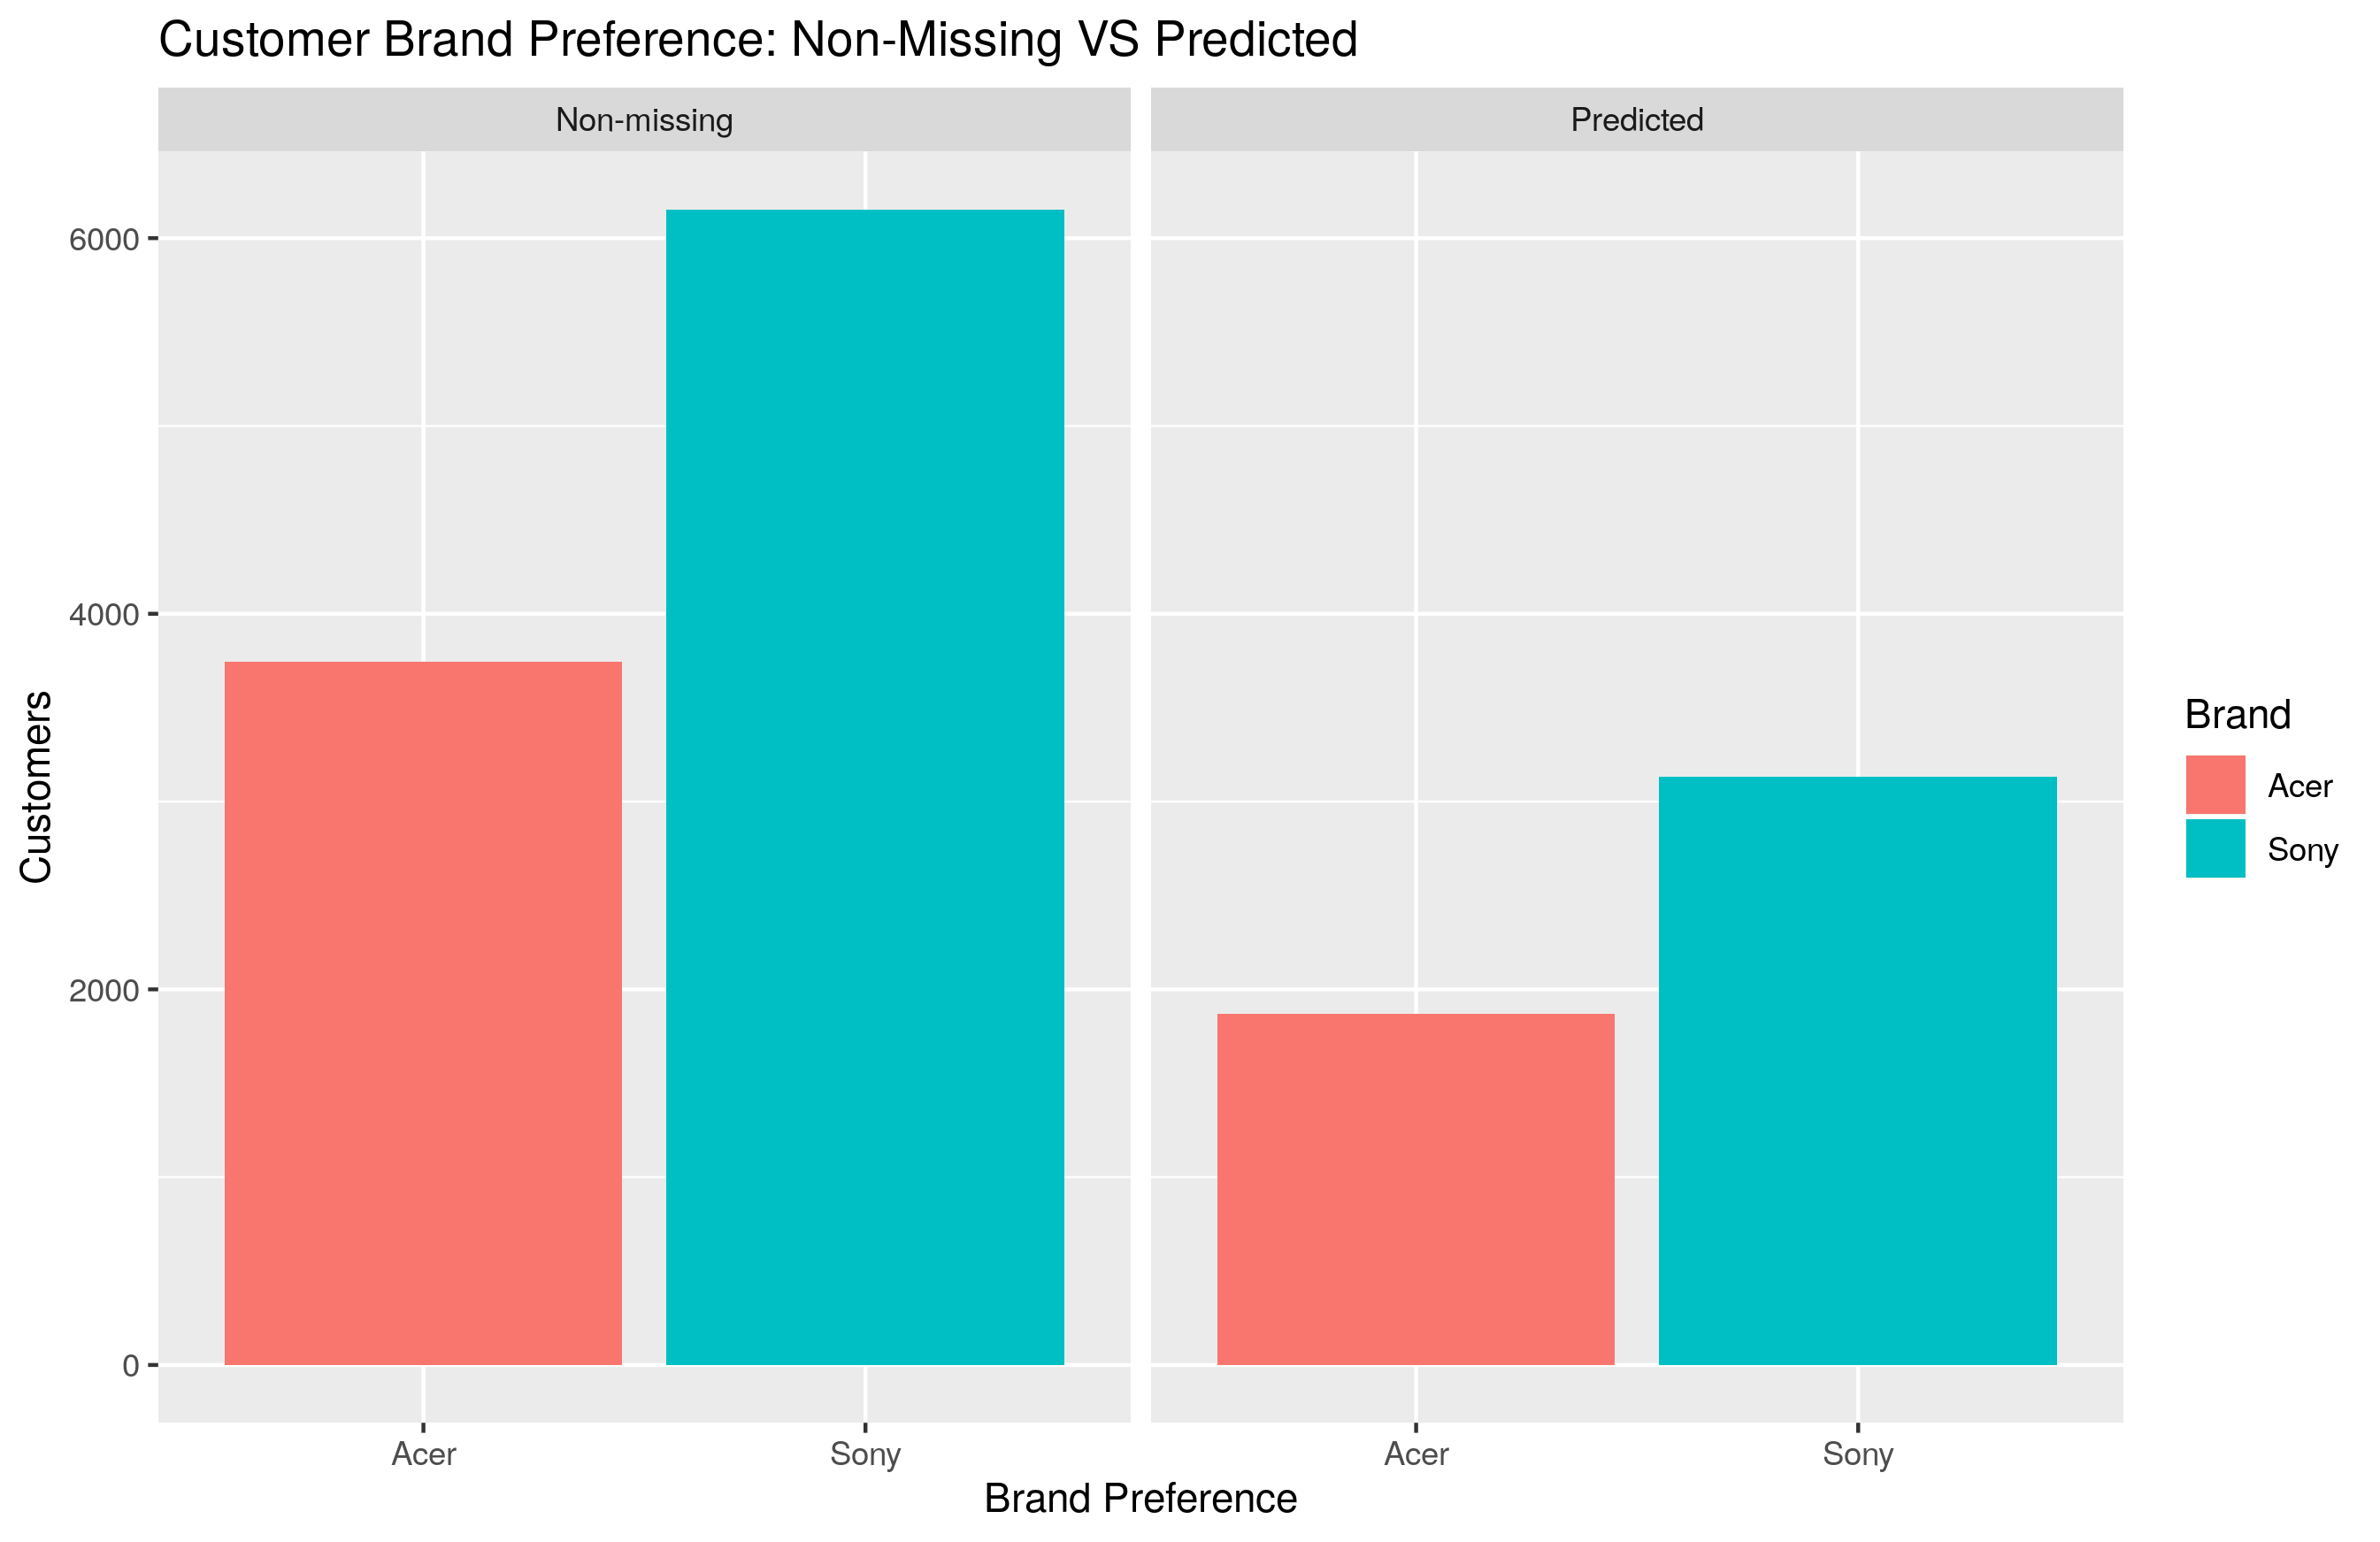
\includegraphics[width=\textwidth,height=\textheight,keepaspectratio]{model_prediction_correlations.png}
%     \par
% }
% \bigskip

This opened up the possibility of trying out an ensemble model that combines all the models, so that
they could compensate for each others weaknesses. This was tried out with the combinations of two models and all
three models. Accuracy of the model improved slightly, but at the same time difference between test accuracy and train
accuracy grew. Because the gains where small, but the change of overfitting much bigger, this venture was abandoned and
a more simple model chosen. In the end C5.0 won, because of the extremely small difference between test and train accuracy.
This model seemed to offer accurate predictions combined with the lowest change of overfitting.

Here are the command line summaries of the models in cross validation state:

\lstinputlisting[float=h,frame=tb,caption=C5.0,label=zebra]{./figures/C5.0_output.txt}
\lstinputlisting[float=h,frame=tb,caption=Extreme Gradient Boosting,label=zebra]{./figures/EGB_output.txt}
\lstinputlisting[float=h,frame=tb,caption=Random Forest,label=zebra]{./figures/RF_output.txt}

\end{document}
